\documentclass{article}

% Präambel
%---| Packages |----------------------------------------------------------------

\usepackage{amsmath}    % Create equations and mathematical expressions.
\usepackage{graphicx}   % Embed captioned figures, images and other graphics.
\usepackage{subcaption} % Display images side-by-side.
\usepackage{setspace}   % Custom spacing for TOC entries.
\usepackage[            % Additional citation options.
    backend = biber,
    style   = ieee
]{biblatex}
\usepackage{hyperref}   % Create Links display URLs.
%---| Settings |----------------------------------------------------------------

% Abbildungen
\graphicspath{{./images}}

% Titelseite
\title{Hello world in LaTeX}
\date{\today}
\author{Henry Behrend}

% The setcounter command can be used to set the TOC's depth to to the following
% values (level meaning everything up to the specified section will be shown):
%   0 - nothing
%   1 - section level
%   2 - subsection level
%   3 - subsubsection level (default)
%   4 - paragraph level
%   5 - subparagraph level

% Inhaltsverzeichnis
\setcounter{tocdepth}{3}

% Quellenverzeichnis
\bibliography{sources}

% Links und URLs
\hypersetup{
    pdfborder  = 0 0 0, % Disable the ugly border around links.
    colorlinks = true,
    linkcolor  = black,
    urlcolor   = blue
}

% Round numbers to two decimal places.
\sisetup{
    round-mode      = places,
    round-precision = 2
}

% For backward compatibility.
\pgfplotsset{compat = 1.18}
%---| Commands |----------------------------------------------------------------

% Personally I use the convention that custom defined commands are Pascal case.
\newcommand{\HelloWorld}{\textbf{Hello, world!}}

% Adds parentheses around a footnote reference for better readability.
\renewcommand*{\thefootnote}{(\arabic{footnote})}

\begin{document}

\pagenumbering{gobble}  % This disables page numbering.
\doublespacing          % This increases spacing between lines.

% Titelseite
\maketitle
\newpage

% Inhaltsverzeichnis
\tableofcontents
\newpage

% Abbildungsverzeichnis
\listoffigures
\newpage

% Tabellenverzeichnis
\listoftables
\newpage

\pagenumbering{arabic}
\singlespacing

% Hauptteil
\section{Section}

\HelloWorld

\subsection{Subsection}

Structuring a document is easy!

\subsubsection{Subsubsection}

Here's some text...

\paragraph{Paragraph}

... and here's some more text ...

\subparagraph{Subparagraph}

... and here's even more text!

\section{Some math and equations}

Displaying math expressions and equations of any kind is effortless in \LaTeX.
This is done by using a package for rendering maths, like \texttt{amsmath} and
then using its \texttt{equation} or \texttt{align} environments for creating
expressions as an extra paragraph. By wrapping the maths inside dollar signs
(\$), you can create inline mathematical expressions.
\begin{center}
    My favorite function is
    $f(x) = \frac{1}{2} \left\lfloor
        mod\left(
            \left\lfloor \frac{y}{17} \right\rfloor
            2^{-17\left\lfloor x \right\rfloor} -
            mod\left( \left\lfloor y \right\rfloor, 17 \right), 2
        \right)
    \right\rfloor$.
\end{center}
Writing more complex or highly nested equations like this can be a bit
cumbersome, so for that case using the
\href{https://latexeditor.lagrida.com/} {Online LaTeX Equation Editor}
might be a good idea.

\paragraph{Enumbered equation}

A normal equation with the \texttt{equation} environment:

\begin{equation}
    1 + 2 = 3
\end{equation}

\paragraph{Unenumbered equation}

An unnumbered equation with the \texttt{equation*} environment:

\begin{equation*}
    1 + 2 = 3
\end{equation*}

\paragraph{Multiline equation}

A multiline equation with alignment can be done with the \texttt{align*}
environment:

\begin{align*}
    1 + 2 &= 3 \\
    1 &= 3 - 2
\end{align*}

\paragraph{Complex equations}

More complex equations can be done with commands like \texttt{frac} for
fractions or \texttt{int} for integrals:

\begin{align*}
    f(x) &= x^2 \\
    g(x) &= \frac{1}{x} \\
    F(x) &= \int^a_b \frac{1}{3}x^3
\end{align*}

These commands may be combined into nested equations such as:

\begin{equation*}
    \frac{1}{\sqrt{x}}
\end{equation*}

\paragraph{Matrices}

Displaying matrices is also possible via the \texttt{matrix} environment,
although only within the above mentioned math environments:

\begin{equation*}
    \begin{matrix}
        1 & 0 \\
        0 & 1
    \end{matrix}
\end{equation*}

If there is a need to surround a matrix with brackets, merely wrapping the
\texttt{matrix} command with bracket characters won't do the trick:

\begin{equation*}
    [
        \begin{matrix}
            1 & 0 \\
            0 & 1
        \end{matrix}
    ]
\end{equation*}

Fortunately, there is a way to scale these brackets up to match the height of
the matrix and, for that matter, other equations too:
This can be done by preceding the opening and closing bracket or parenthesis by
the \texttt{left} and \texttt{right} command respectively.

\begin{equation*}
    \left[
        \begin{matrix}
            1 & 0 \\
            0 & 1
        \end{matrix}
    \right]
\end{equation*}

\begin{equation*}
    \left(\frac{1}{\sqrt{x}}\right)
\end{equation*}

\newpage
\section{Captioned figures and images}

Embedding captioned images and figures into your document by using the
\texttt{figure} environment from the \texttt{graphicx} package:

% The image placement can be controlled by setting the float parameter to one of
% the following values:
%   h (here)     - location in code equals location in the document
%   t (top)      - top of the page
%   b (bottom)   - bottom of the page
%   p (page)     - on a separate page
%   ! (override) - force the specified location (analogous to !important in CSS)
%
% Even stricter placement can be achieved by using the float package's H option.

\begin{figure}[h!]
    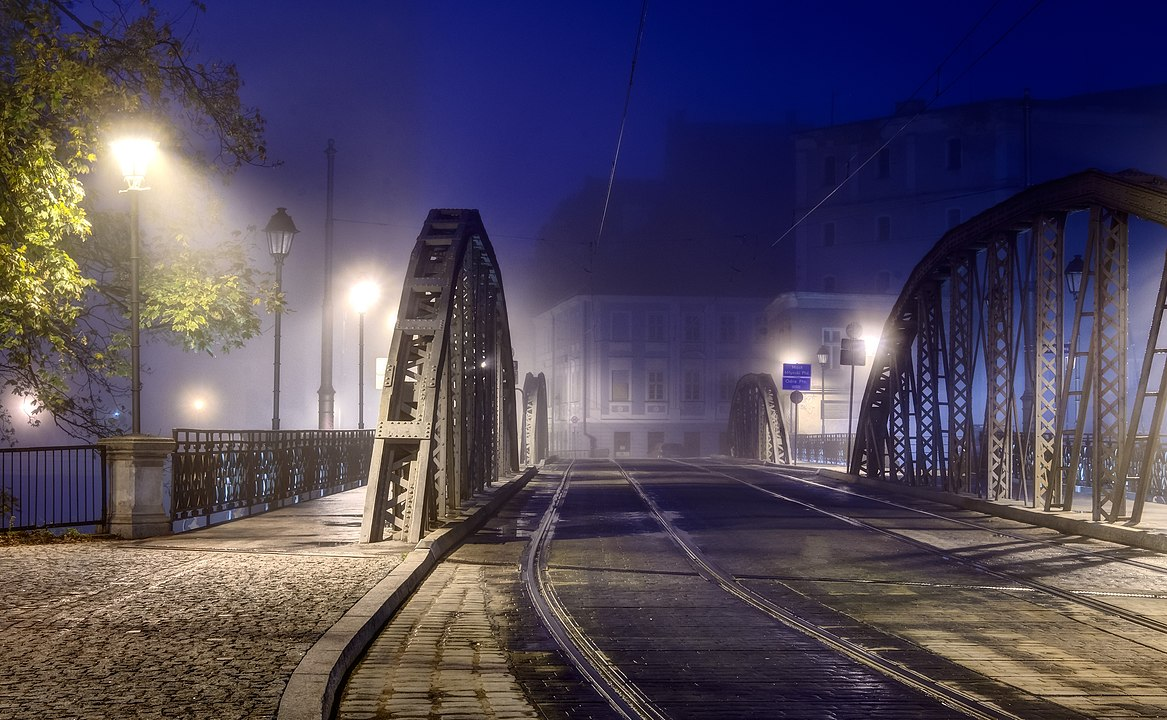
\includegraphics[width=\linewidth]{bridge.jpg}
    \caption{A Bridge.}
    \label{fig:bridge}
\end{figure}

% Most of this paragraph was taken from https://latex-tutorial.com.
Figure \ref{fig:bridge} shows the Mlynski Bridge in Wroclaw. Sometimes when
writing a document, adding single images is not optimal, especially when the
reader is supposed to compare several results or graphs. In such situations, it
might be necessary to use a different environment, called subfigure. The
\texttt{subfigure} environment allows you to place multiple images at a certain
location next to each other and the usage is pretty straightforward:

\begin{figure}[h!]
    \centering
    \begin{subfigure}[b]{0.4\linewidth}
        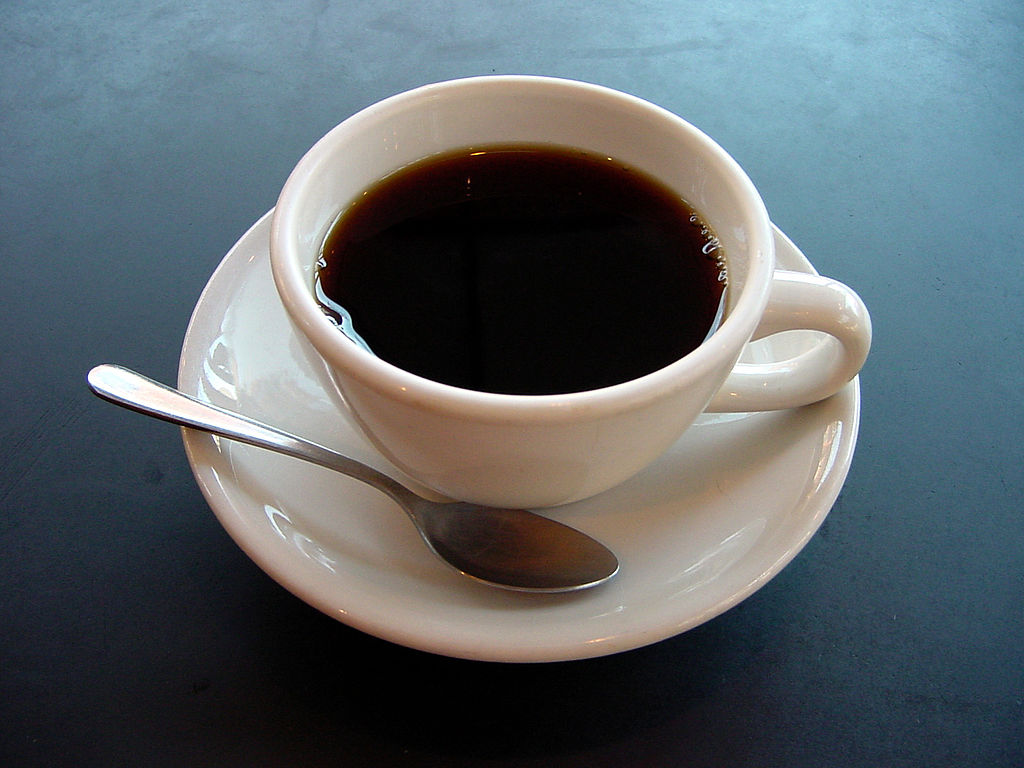
\includegraphics[width=\linewidth]{coffee.jpg}
        \caption{A cup of coffee.}
    \end{subfigure}
    \begin{subfigure}[b]{0.4\linewidth}
        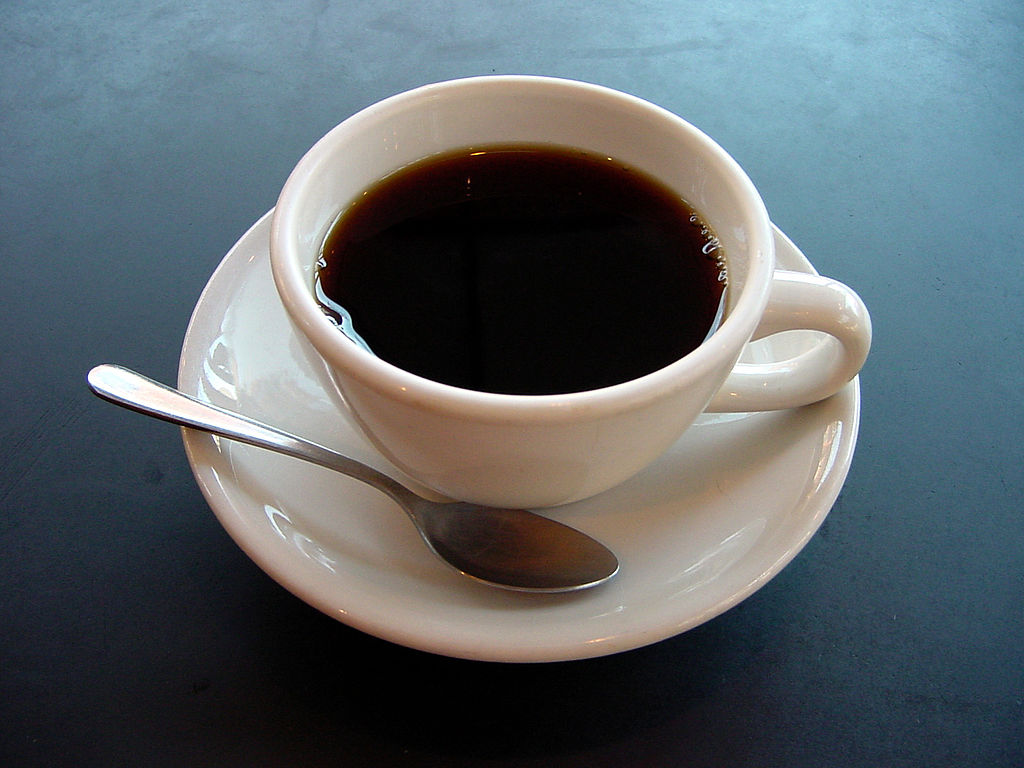
\includegraphics[width=\linewidth]{coffee.jpg}
        \caption{Another cup of coffee.}
    \end{subfigure}
    \caption{Two cups of coffee side by side.}
    \label{fig:coffee}
\end{figure}

\section{Table of contents (TOC)}

The TOC can be generated automatically via the \texttt{tableofcontents} command.
By default, sections, subsections and subsubsections are displayed there, this
called the TOC's depth. The depth can be changed via the \texttt{setcounter}
command by setting its first argument to \texttt{tocdepth} and the second
argument to the desired value.

It is also possible to set the depth locally rather than for the whole document
by calling the \texttt{addtocontents} command before declaring the sections to
be affected by the local depth setting. An example can be seen right below:

\addtocontents{toc}{\setcounter{tocdepth}{1}}

\section{A section with a custom depth value for the TOC}

The following subsection and subsubsection should not be part of the TOC.

\subsection{I'm not part of the TOC}

\subsubsection{Me neither}

% This resets the TOC's depth value, since 3 is the default.
\addtocontents{toc}{\setcounter{tocdepth}{3}}

\section{A new section with the global depth value}

\subsection{I'm in the TOC again!}

\section{Bibliography and citations}

Managing sources and citations is really easy with \LaTeX. There are external
tools for creating and maintaining bibliographies, like \textit{Biblatex} or
\textit{Bibtex} in case of this particular project.

\subsection{Creating the bibliography}

The bibliography is created by calling the \texttt{bibliography} command and the
preferred citation style is set via the \texttt{bibliographystyle} command.
Bibtex requires the creation of a \texttt{.bib} file, which holds the
bibliographic information. To see how such a file is structured, take a look at
the file \texttt{bibliography.bib} located in the project's root folder.

\subsection{Citation}

After setting up the bibliography, the \texttt{cite} command is used to cite,
refer or quote the source material contained in the bibliography. A really good
book for example would be \autocite{mindstorms}.

\subsection{Biblatex}

Although Biblatex is quite good for the above mentioned use cases, it is limited
to basic citation styles. If citing literature in footnotes is necessary for
example, Biblatex isn't really helpful for that kind of task and should be
swapped in favor of a more versatile alternative like Biblatex. Biblatex can
and will be used here on top of Bibtex and thus extends its the feature set. It
has to be made available first by including the \texttt{biblatex} package. Then,
the used \texttt{.bib} file has to be specified with the \texttt{bibliography}
command inside the preamble. Creating the bibliography is done via the
\texttt{printbibliography} command where we created the bibliography before.
Additionally, citations are created by calling \texttt{autocite} instead of
\texttt{cite}.

Footnotes can be created by either setting the \texttt{style} package option to
\texttt{verbose-trad2} or any other citation style which includes footnotes for
that matter. All available values for the \texttt{style} can be found
\href{https://ctan.joethei.xyz/macros/latex/contrib/biblatex/doc/biblatex.pdf#subsection.3.3}{here}.

\section{Footnotes}

Footnotes can be added to the current page by calling the \texttt{footnote}
command. Additionally, the footnotes content can be referenced by assigning it a
\texttt{label} and referencing it somewhere else with \texttt{ref}. In this
sentence, I refer to footnote content\footnote{Hello,footnotes!} in order to
explain a scientific term for example.

Light rays travel at $c$\footnote{\label{speed_of_light}The speed of light in a
vacuum, defined to be $299792458\frac{m}{s}$.}. Referencing a footnote at some
other point in the document looks like this: You cannot change
\ref{speed_of_light}, it is constant.

\newpage
\section{Tables and tabular environments}

Creating tables is very different to text editors or other word processors like
Microsoft Word, but once you get the hang of it, also pretty straightforward and
simple. Below is a basic example of a table created entirely with \LaTeX. 

% Column alignment is done in the tabular enviroment's first argument.
% Individual alignment values are separated by a horizontal line character (|)
% for a single vertical line or two (||) for a double vertical line.
% The column alignment can take one of the following values:
%   l        - left-justified column
%   r        - right-justified column
%   c        - centered column
%   p{width} - paragraph column with top-aligned text
%   b{width} - paragraph column with bottom-aligned text
%   m{width} - paragraph column with middle-aligned text
%
% If the column alignment is the same for multiple columns the following
% express can be used instead:
%   *{amount}{format}
% For example, *{3}{|l}| is equivalent to |l|l|l|.

\begin{table}[h!]
    \begin{center}
        \begin{tabular}{l|c|r}
            \textbf{Value 1}    & \textbf{Value 2}  & \textbf{Value 3} \\
            $\alpha$            & $\beta$           & $\gamma$ \\
            \hline % A horizontal line separating table head and table body.
            1   & 1110.1      & a \\
            2   & 10.1        & b \\
            3   & 23.113231   & c \\
        \end{tabular}
        \label{tab:standard}
        \caption{My first table.}
    \end{center}
\end{table}

The first table is not optimal. The numeric values in the second column aren't
aligned at the decimal point. To fix this, we can the \texttt{siunitx} package.

% Same table as before, but using the 'S' alignment provided by the siunitx
% package.
\begin{table}[h!]
    \begin{center}
        \begin{tabular}{l|S|r}
            \textbf{Value 1}    & \textbf{Value 2}  & \textbf{Value 3} \\
            $\alpha$            & $\beta$           & $\gamma$ \\
            \hline
            1   & 1110.1      & a \\
            2   & 10.1        & b \\
            3   & 23.113231   & c \\
        \end{tabular}
        \label{tab:aligned_values}
        \caption{A table where numbers are aligned at the decimal point.}
    \end{center}
\end{table}

Once a table is set up, adding additional rows is easy. Just copy the previous
row and change its values according to your needs. Adding extra columns is
possible too, but not as easy, since adding a column requires expanding the
existing rows by another cell, i.e. an \texttt{\&} and optionally a value.

\subsection{Multirows and -columns}

Cells spanning multiple rows can be created with the \texttt{multirow} command.
The command takes 3 arguments, the first being the number of rows the multirow
should take up, the second determining its width (can be set to an asterisk
\texttt{*} for autoscaling) and the last parameter being the rows content, or,
more accurately, the value of the multirow's first column.
Note that for the next $n$ rows the multirow spans across the first column value
is omitted. Take a look at the source code for a comprehensive example of how
\texttt{multitow} is used.

\newpage % Place tables on the new page because they don't fit anymore.

\begin{table}[h!]
    \begin{center}
        \begin{tabular}{l|S|r}
            \textbf{Value 1}    & \textbf{Value 2}  & \textbf{Value 3} \\
            $\alpha$            & $\beta$           & $\gamma$ \\
            \hline
            \multirow{2}{*}{12}
                & 1110.1    & a \\
                & 10.1      & b \\
            \hline
            3   & 23.113231 & c \\
            4   & 23.113231 & d \\   
        \end{tabular}
        \label{tab:multirow}
        \caption{A multirow table.}
    \end{center}
\end{table}

Similar to \texttt{multirow} there's a command to create cells spanning more
than a single column called \texttt{multicolumn}. Like \texttt{multirow}, the
command takes the number of columns as its first and the content as its third
argument. But unlike \texttt{multirow}, the second argument sets the
multicolumn's alignment with values similar to the \texttt{tabular}
environment's alignment parameter.

\begin{table}[h!]
    \begin{center}
        \begin{tabular}{l|S|r}
            \textbf{Value 1}    & \textbf{Value 2}  & \textbf{Value 3} \\
            $\alpha$            & $\beta$           & $\gamma$ \\
            \hline
            \multicolumn{2}{c|}{12}
                            & a \\
            \hline
            2   & 10.1      & b \\
            3   & 23.113231 & c \\
            4   & 23.113231 & d \\
        \end{tabular}
        \label{tab:multicol}
        \caption{A multicolumn table.}
    \end{center}
\end{table}

Both commands my be combined to create cells spanning multiple rows and columns:

\begin{table}[h!]
    \begin{center}
        \begin{tabular}{l|S|r}
            \textbf{Value 1}    & \textbf{Value 2}  & \textbf{Value 3} \\
            $\alpha$            & $\beta$           & $\gamma$ \\
            \hline
            \multicolumn{2}{c|}{\multirow{2}{*}{1234}}
                            & a \\
            \multicolumn{2}{c|}{} % Creates an empty multirow as placeholder.
                            & b \\
            \hline
            3   & 23.113231 & c \\
            4   & 23.113231 & d \\
        \end{tabular}
        \label{tab:multiboth}
        \caption{A table with a $2 \times 2$ cell.}
    \end{center}
\end{table}

\newpage

\subsection{Customizing tables}

Leveraging the extra features provided by the \texttt{booktabs} package, we can
create better looking tables. Using the \texttt{toprule}, \texttt{middlerule}
and \texttt{bottomrule} commands, table sections can be separated more clearly.

\begin{table}[h!]
    \begin{center}
        \begin{tabular}{l|S|r}
            \toprule
            \textbf{Value 1}    & \textbf{Value 2}  & \textbf{Value 3} \\
            $\alpha$            & $\beta$           & $\gamma$ \\
            \midrule
            1   & 1110.1      & a \\
            2   & 10.1        & b \\
            3   & 23.113231   & c \\
            \bottomrule
        \end{tabular}
        \label{tab:pretty}
        \caption{A better looking table.}
    \end{center}
\end{table}

Normally, when a table doesn't fit on a single page, it gets cropped at the
bottom. To prevent this from happening, the \texttt{longtable} package can be
used to create tables that span multiple pages. A solution for a table spanning
too many columns would be to display it rotated by 90 degrees counterclockwise.
This can be achieved with the \texttt{rotating} package by creating landscape
tables.

\subsection{Importing tables from CSV files}

% Quellenverzeichnis
\newpage
\printbibliography

\end{document}